%
% The first command in your LaTeX source must be the \documentclass command.
\documentclass[acmlarge,screen]{acmart}
% --------------------------------------------------------------
% Code Formatting
% --------------------------------------------------------------
\usepackage{listings}
\usepackage{color}

\definecolor{codegreen}{rgb}{0,0.6,0}
\definecolor{codegray}{rgb}{0.5,0.5,0.5}
\definecolor{codepurple}{rgb}{0.58,0,0.82}
\definecolor{backcolour}{rgb}{0.95,0.95,0.92}

\lstdefinestyle{mystyle}{
	backgroundcolor=\color{backcolour},   
	commentstyle=\color{codegreen},
	keywordstyle=\color{magenta},
	numberstyle=\tiny\color{codegray},
	stringstyle=\color{codepurple},
	basicstyle=\footnotesize,
	breakatwhitespace=false,         
	breaklines=true,                 
	captionpos=b,                    
	keepspaces=true,                 
	numbers=left,                    
	numbersep=5pt,                  
	showspaces=false,                
	showstringspaces=false,
	showtabs=false,                  
	tabsize=2
}

\lstset{style=mystyle}

%
% defining the \BibTeX command - from Oren Patashnik's original BibTeX documentation.
\def\BibTeX{{\rm B\kern-.05em{\sc i\kern-.025em b}\kern-.08emT\kern-.1667em\lower.7ex\hbox{E}\kern-.125emX}}

% Rights management information.
% This information is sent to you when you complete the rights form.
% These commands have SAMPLE values in them; it is your responsibility as an author to replace
% the commands and values with those provided to you when you complete the rights form.
%
% These commands are for a PROCEEDINGS abstract or paper.
\copyrightyear{2019}
\acmYear{2019}
\setcopyright{acmlicensed}
\acmConference[SIGGRAPH 2019]{SIGGRAPH 2019: THE 46TH INTERNATIONAL CONFERENCE & EXHIBITION ON COMPUTER GRAPHICS & INTERACTIVE TECHNIQUES}{28 July - 1 August, 2019}{Los Angeles, California}
\acmBooktitle{SIGGRAPH 2019: THE 46TH INTERNATIONAL CONFERENCE & EXHIBITION ON COMPUTER GRAPHICS & INTERACTIVE TECHNIQUES, 28 July - 1 August, 2019, Los Angeles, CA}
\acmPrice{15.00}
\acmDOI{10.1145/1122445.1122456}
\acmISBN{978-1-4503-9999-9/18/06}

%
% These commands are for a JOURNAL article.
%\setcopyright{acmcopyright}
%\acmJournal{TOG}
%\acmYear{2019}\acmVolume{37}\acmNumber{4}\acmArticle{111}\acmMonth{8}
%\acmDOI{10.1145/1122445.1122456}

%
% Submission ID.
% Use this when submitting an article to a sponsored event. You'll receive a unique submission ID from the organizers
% of the event, and this ID should be used as the parameter to this command.
%\acmSubmissionID{123-A56-BU3}

%
% The majority of ACM publications use numbered citations and references. If you are preparing content for an event
% sponsored by ACM SIGGRAPH, you must use the "author year" style of citations and references. Uncommenting
% the next command will enable that style.
%\citestyle{acmauthoryear}

%
% end of the preamble, start of the body of the document source.
\begin{document}

%
% The "title" command has an optional parameter, allowing the author to define a "short title" to be used in page headers.
\title{Reconstructing the MRI Aesthetic in Digital Holography}
\subtitle{A review of various techniques to identify the optimal approach for medical digital holograms}

%
% The "author" command and its associated commands are used to define the authors and their affiliations.
% Of note is the shared affiliation of the first two authors, and the "authornote" and "authornotemark" commands
% used to denote shared contribution to the research.
\author{Michael Page}
\email{mpage@faculty.ocadu.ca}
\orcid{1234-5678-9012}
\affiliation{%
  \institution{OCAD University}
  \streetaddress{205 Richmond Street West, Lower Level}
  \city{Toronto}
  \state{Ontario}
  \postcode{M5V 1V3}
}

\author{Jawa El Khash}
\email{jelkhash@faculty.ocadu.ca}
\orcid{1234-5678-9012}
\affiliation{%
  \institution{OCAD University}
  \streetaddress{205 Richmond Street West, Lower Level}
  \city{Toronto}
  \state{Ontario}
  \postcode{M5V 1V3}
}

\author{Adriana Menghi}
\email{amenghi@faculty.ocadu.ca}
\orcid{1234-5678-9012}
\affiliation{%
  \institution{OCAD University}
  \streetaddress{205 Richmond Street West, Lower Level}
  \city{Toronto}
  \state{Ontario}
  \postcode{M5V 1V3}
}

\author{Mario Garingo}
\email{mgaringo@ocadu.ca}
\orcid{1234-5678-9012}
\affiliation{%
  \institution{OCAD University}
  \streetaddress{205 Richmond Street West, Lower Level}
  \city{Toronto}
  \state{Ontario}
  \postcode{M5V 1V3}
}

\author{Marcus A. Gordon}
\email{mgordon@faculty.ocadu.ca}
\orcid{1234-5678-9012}
\affiliation{%
  \institution{OCAD University}
  \streetaddress{205 Richmond Street West, Lower Level}
  \city{Toronto}
  \state{Ontario}
  \postcode{M5V 1V3}
}

%
% By default, the full list of authors will be used in the page headers. Often, this list is too long, and will overlap
% other information printed in the page headers. This command allows the author to define a more concise list
% of authors' names for this purpose.
\renewcommand{\shortauthors}{Page and Gordon, et al.}

%
% The abstract is a short summary of the work to be presented in the article.
\begin{abstract}

In this research we propose a methodology that uses existing software tools to encode the MRI data into a multitude of two dimensional images. The proposed solution is the creation of a process that enables MRI data to be converted directly into a digital, holographic, print-ready form that requires no further processing and little to no human intervention.
\end{abstract}

%
% The code below is generated by the tool at http://dl.acm.org/ccs.cfm.
% Please copy and paste the code instead of the example below.
%
\begin{CCSXML}
<ccs2012>
<concept>
<concept_id>10010147.10010178.10010224.10010226.10010236</concept_id>
<concept_desc>Computing methodologies~Computational photography</concept_desc>
<concept_significance>500</concept_significance>
</concept>
<concept>
<concept_id>10010147.10010178.10010224.10010245.10010247</concept_id>
<concept_desc>Computing methodologies~Image segmentation</concept_desc>
<concept_significance>500</concept_significance>
</concept>
<concept>
<concept_id>10003456.10003462.10003602.10003608</concept_id>
<concept_desc>Social and professional topics~Medical technologies</concept_desc>
<concept_significance>500</concept_significance>
</concept>
<concept>
<concept_id>10010147.10010178.10010224.10010226.10010239</concept_id>
<concept_desc>Computing methodologies~3D imaging</concept_desc>
<concept_significance>500</concept_significance>
</concept>
<concept>
<concept_id>10010147.10010371.10010387.10010393</concept_id>
<concept_desc>Computing methodologies~Perception</concept_desc>
<concept_significance>300</concept_significance>
</concept>
<concept>
<concept_id>10010147.10010371.10010396.10010401</concept_id>
<concept_desc>Computing methodologies~Volumetric models</concept_desc>
<concept_significance>300</concept_significance>
</concept>
<concept>
<concept_id>10010147.10010371.10010372.10010374</concept_id>
<concept_desc>Computing methodologies~Ray tracing</concept_desc>
<concept_significance>100</concept_significance>
</concept>
<concept>
<concept_id>10010147.10010371.10010387.10010394</concept_id>
<concept_desc>Computing methodologies~Graphics file formats</concept_desc>
<concept_significance>500</concept_significance>
</concept>
<concept>
<concept_id>10010147.10010341.10010349.10010364</concept_id>
<concept_desc>Computing methodologies~Scientific visualization</concept_desc>
<concept_significance>300</concept_significance>
</concept>
<concept>
<concept_id>10010405.10010469.10010474</concept_id>
<concept_desc>Applied computing~Media arts</concept_desc>
<concept_significance>500</concept_significance>
</concept>
</ccs2012>
\end{CCSXML}

\ccsdesc[500]{Computing methodologies~Computational photography}
\ccsdesc[500]{Computing methodologies~Image segmentation}
\ccsdesc[500]{Social and professional topics~Medical technologies}
\ccsdesc[500]{Computing methodologies~3D imaging}
\ccsdesc[300]{Computing methodologies~Perception}
\ccsdesc[300]{Computing methodologies~Volumetric models}
\ccsdesc[100]{Computing methodologies~Ray tracing}
\ccsdesc[500]{Computing methodologies~Graphics file formats}
\ccsdesc[300]{Computing methodologies~Scientific visualization}
\ccsdesc[500]{Applied computing~Media arts}

%
% Keywords. The author(s) should pick words that accurately describe the work being
% presented. Separate the keywords with commas.
\keywords{digital holography, graphics pipeline, volume rendering, linear color, MRI}

%
% A "teaser" image appears between the author and affiliation information and the body
% of the document, and typically spans the page.
%%\begin{teaserfigure}
%%  \includegraphics[width=\textwidth]{sampleteaser}
%%  \caption{Seattle Mariners at Spring Training, 2010.}
%%  \Description{Enjoying the baseball game from the third-base seats. Ichiro Suzuki preparing to bat.}
%%  \label{fig:teaser}
%%\end{teaserfigure}

%
% This command processes the author and affiliation and title information and builds
% the first part of the formatted document.
\maketitle

% --------------------------------------------------------------
% Introduction
% --------------------------------------------------------------
\newpage
\section{Introduction}
\newpage
\subsection{}

% --------------------------------------------------------------
% Research Question
% --------------------------------------------------------------
\newpage
\section{Research Questions}
Is there a linear transformation that takes MRI images and creates holographic image stacks for printing?


% --------------------------------------------------------------
% Lit Review
% --------------------------------------------------------------
\newpage
\section{Literature Review}
\input{sections/litReview/litReview.tex}

% --------------------------------------------------------------
% Methodology
% --------------------------------------------------------------
\newpage
\section{Methodology}
In this section we will focus on the overall pipeline of the project as described in Figure \ref{fig:pipeline}.  This section will be divided into 4 sections: segmentation, generating 3D models or geometry, image stage generation, and finally digital holograms. 

\begin{figure}[H]
  \centering
  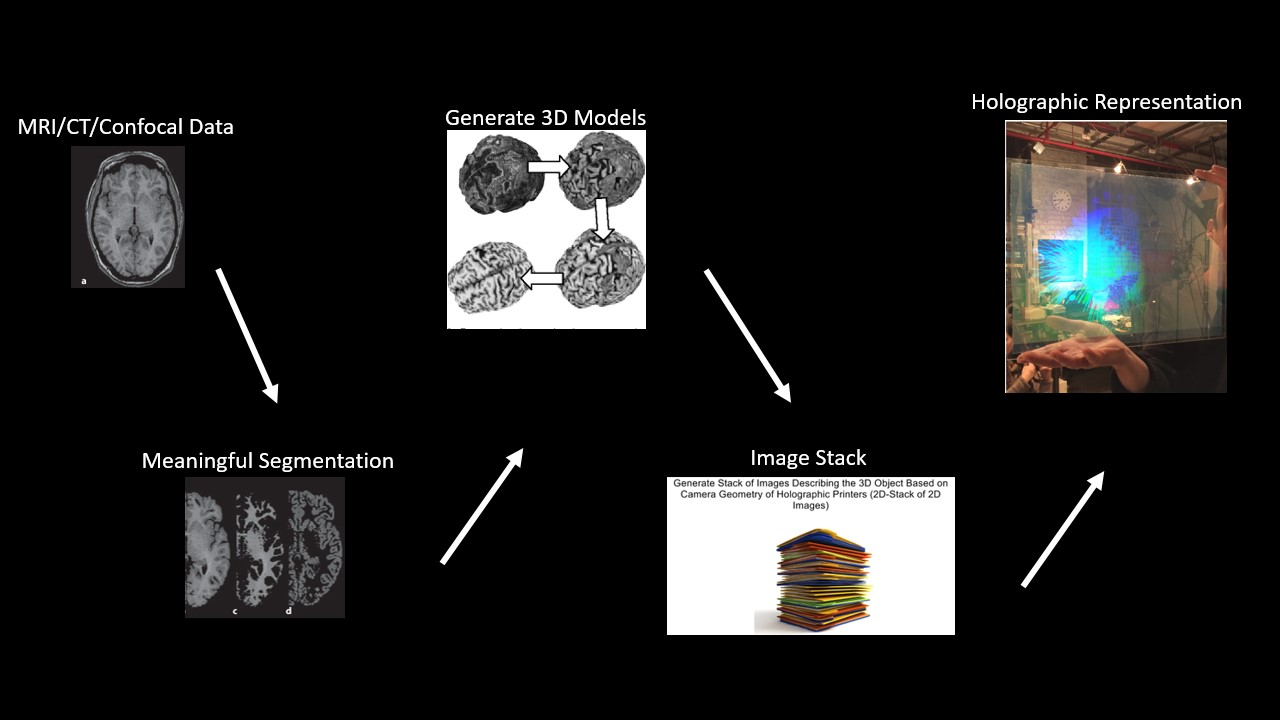
\includegraphics[width=\linewidth]{img/pipeline.jpg}
  \caption{General pipeline from medical image to a digital holographic print.}
  \label{fig:pipeline}
\end{figure}

\begin{figure}[H]
  \centering
  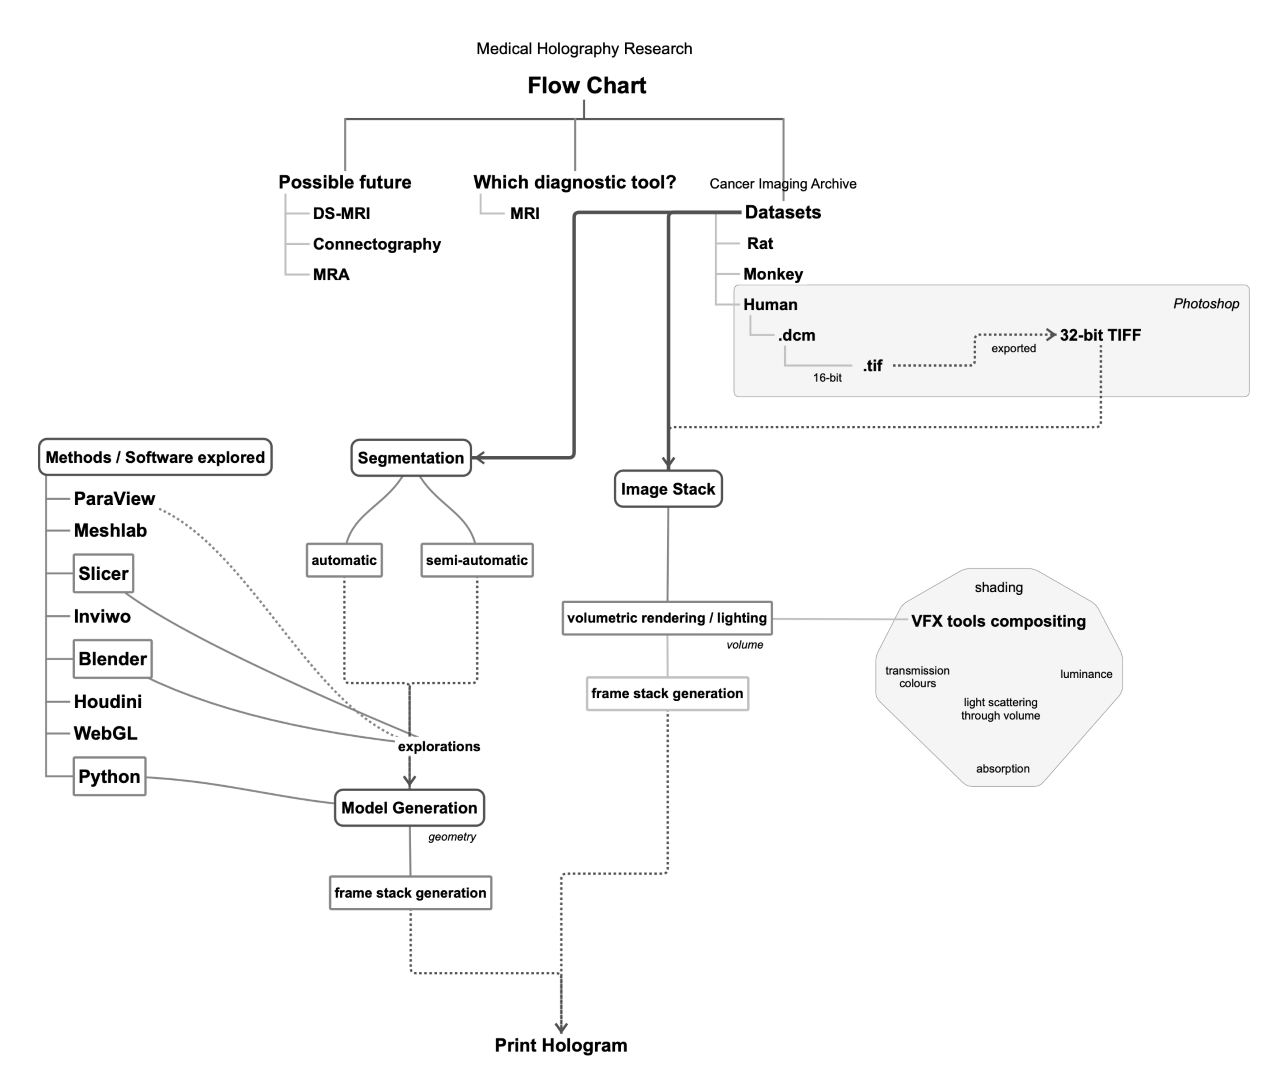
\includegraphics[width=\linewidth]{img/detailedFlowChart.png}
  \caption{Detailed pipeline of our medical image to a digital holographic print research methodology.}
  \label{fig:detailedPipeline}
\end{figure}




\subsection{Segmentation}

The main objective of this project was to determine if the physicians/clinicians/technicians are able to obtain more meaningful information when given more depth information through a holographic print.  To give this type of information, structural patterns within the model must be apparent. To achieve this we used a data-set of a human brain containing a tumor. We believe that the depth information inherently found in holography, will make the location of the tumor become apparent.  As an intermediate step we need to develop geometry for each of the salient structures of the brain, mainly the white and gray matter, as well as the tumor and other abnormal tissues surrounding the tumor.  This is where segmentation algorithms are needed.\\

There are several different approaches that have been found throughout the literature \cite{pham2000current}.  But they all stem from the same set of core ideas.  In this project we explored both automatic and semi-automatic methods.

\subsubsection{Automatic}

One of our ultimate goal of the project is to use existing software and have a file-print process in which the MRI data is generated directly into a holographic print without any human intervention.  This automatic approach from MRI to holographic print needs automatic annotation and segmentation of the MRI data.  Current methods include the annotation and segmentation of each of the slices. This is inefficient and also time consuming. In this section we will explore the possibility of automating this step using transfer leaning and 3D U-Net dense volumetric segmentation\cite{cciccek20163d}.\\

One of the main issues using deep learning methods in the medical field, is the lack of a large enough sample size for the network to fully stabilize the weights and biases.  To overcome this issue it is often the case that we have to use transfer learning techniques using pre-trained networks.  In this project we explored the possibility of using inductive transfer learning\cite{pan2010survey} and a pre-trained network found in the work of \cite{cciccek20163d}.  Using transfer learning, instead of starting the learning process from the beginning, the learning process starts from patterns that have been learned when solving a different or similar problem. In this way, we essentially utilize previous learning's from the pre-trained network and apply them to our dataset.\\

The work done by \cite{cciccek20163d} expands the work previously achieved by \cite{ronneberger2015u} but using 3D volumetric data.  There is an added dimension of depth in all filters and weights in the U-Net architecture.  The depth information comes from the slice information in the MRI. During the encoder or down sampling portion of the architecture two 3 x 3 x 3 convolutions were performed followed by a rectified linear unit (ReLu).  This was followed up by a single 2 x 2 x 2 max pooling with strides of 2 in each dimension.  In the synthesis or up-convolution path a 2 x 2 x 2 with strides of 2 in each dimension was used followed by the mirrored 3 x 3 x 3 convolution with ReLu.  To reduce bottle-necking doubling the channels was done before each max pooling layer.  In the last layer a 1 x 1 x 1 x 1 convolution was used for the output layer for each of the labeled cases white matter, gray matter, tumor and abnormal tissue. The last layer used a weighted softmax loss function.  Note that the input layer was 256 x 256 x 118.

\begin{figure}[H]
  \centering
  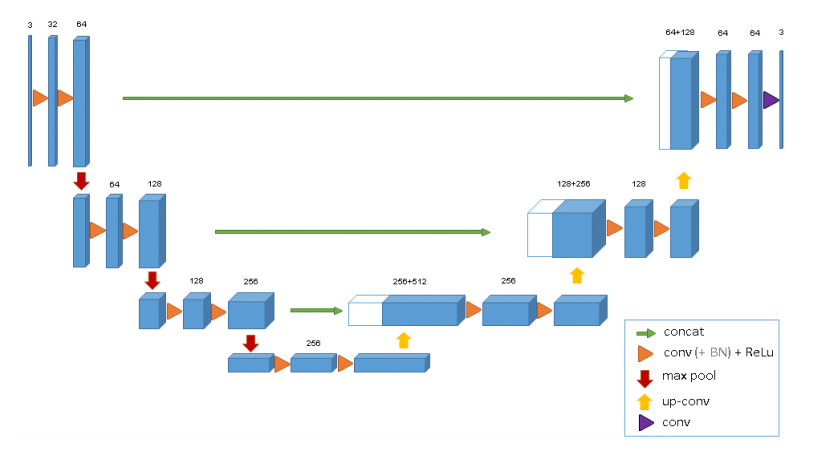
\includegraphics[width=\linewidth]{img/volumetricUNetArchitecture.PNG}
  \caption{UNet architecture used in Cicek et.el. \cite{cciccek20163d}}
  \label{fig:uNet}
\end{figure}

In theory this approach would have worked but the data used by \cite{cciccek20163d} was too different from the data we are using, so the transfer learning did not give us the adequate segmentation we wanted.  Due to the limited time of the project this was abandoned and semi-automatic techniques were more focused as they are more intuitive and don't require a large sample size.  In the future we would like to pursue this approach as this would be more akin to our ultimate goal of the file-print process.


\subsubsection{Semi-Automatic}

Since the brain consists of known tissue types such as white and gray matter, bone and spinal fluid, the intuitive approach would be to classify these based on intensity values of the pixels on the MRI \cite{atkins1998fully}.  The problem arises when there are overlapping tissues in which case the intensity values of each pixel will be miss classified as one of the known tissue types \cite{undeman2003fully}.  This is why current MRI segmentation is not fully automated and radiologists are needed to help the computer identify which pixels are wrong and correct it. To combat this issue, there are some algorithms such as the one proposed by \cite{lenroot2006brain} whereby they use pre-segmented brain template and perform image registration and automatically identify the troublesome pixels and fix the labels accordingly.\\  

However necessary, the main purpose of this project is not on segmentation rather exploring the depth information of the digital holographic print.  So we will not use complex segmentation techniques, instead we will use the more intuitive approach of pixel classification using multithresholding (MT) techniques \cite{sahoo1988survey} in combination with region growing approaches\cite{adams1994seeded}.\\

The overall goal of MT is to generate masks which partition the image into our desired segmented areas.  To do this a histogram is first generated to identify the threshold ranges of each tissue type.  The segmentation is achieved by grouping similar pixel intensities together akin to quantizing the image.  But in this case the quantization levels are not constant. This is clearly seen in figure \ref{fig:mriHistogram}.  In the MRI you can see three distinct colours which corresponds to the white and gray matter (WM,GM) and also the cerebral fluid (CSF).  The histogram distributions show 3 distinct peak which corresponds to these tissue types.

\begin{figure}[H]
  \centering
  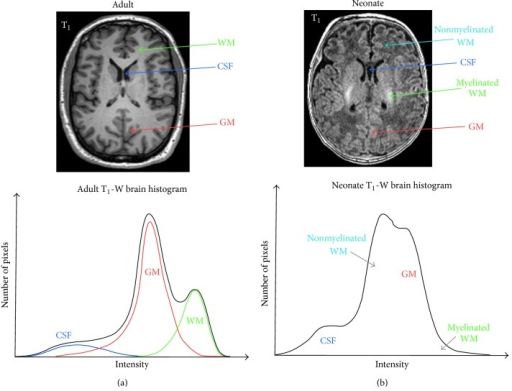
\includegraphics[width=\linewidth]{img/mriHistogram.png}
  \caption{MRI and pixel intensity histogram distribution.}
  \label{fig:mriHistogram}
\end{figure}

Notice the problem described earlier, there are overlapping pixels in the histogram that can be in either of the 3 labeled tissue classes.  We will combat this problem by introducing a region growing approach.\\

Region growing is a simple yet effective technique which samples and extracts a region of the image by connecting similar pixels together. Though very similar to thresholding, this introduces a fuzzy thresholding approach rather than categorical quantization.  The fuzzy approach comes about through the corporation of both the intenisty and edges of the image. The main step is to add a seed point which is manually selected, and from this point connect all the pixels surrounding it together and label that region accordingly.  In the literature this is often done for tumor and lesion segmentation\cite{guliato1998segmentation}. The main disadvantage of this approach is the resultant mask can be very noisy causing the extracted region to have holes and disconnected regions.  To remedy this affect we applied morphological filters\cite{mendiola2007morphological}.\\

Our python implementation can be found in Appendix \ref{sec:appendixPythonFunction}.
 \subsection{Generating Geometry}

\subsubsection{Marching Cube Algorithm}
Given a set of slices of a 3D image we can identify the vertices and edges by looking at the edges of the masks for each segmentation.  Once this is accomplished a marching cube algorithm can be used to create a 3D surface by creating triangular connections between the vertices. This is done by performing an exhaustive iterative search throughout the entire image plane\cite{lorensen1987marching}.\\  

Intuitively, the algorithm fists divides the 3D region into cubes.  For each cube you compute weather an edge or a vertex lies within the cube and where it passes through the edge of the cube. If these conditions are met cube is part of the geometry.  After this is done you triangulate the surface to reduce redundancies and also to create a mesh. This is done by identifying where the object passes through the edges of the cube.  To create the isosurface you connect these junctions together and remove redundant connections.\\

Smoothing can also take part here but Trevor suggested not doing so because in the medical field altering the data is not acceptable.\\

Our python implementation can be found in Appendix \ref{sec:appendixPythonFunction}.

\subsubsection{MRI Volume}
An additional method to be explored is in the generating of a three dimensional volume of the brain tumor progression.  A two-step process that involves creating an image texture from DICOM files, and applying it to a simple 1x1x1 cube geometry, creating a volumetric texture \cite{voxeldata2019}, to generate an MRI volume. As a volume, we get greater aesthetic variance than with surface materials alone, but with less control of particular vertex colours than dealing with geometry.  The impact here is that segmentation of the volume becomes similar to segmentation applied to the MRI slices in traditional medical imaging analysis cases.  We estimate that as a digital hologram this would eventually provide greater flexibility in colour variation through volumetric scattering and absorption.\\

To test this hypothesis, we first looked at our tool of choice for this experiment: Blender, an open source 3D creation environment.  It supports an entire beginning to end 3D pipeline, and is often used for scientific visualization \cite{garate2017voxel} \cite{kent20143d}. Using the attributes of volume rendering in Blender, an experiment for the volumetric rendering of our MRI dataset could be carried out by setting values to attributes such as emission, density, transparency, and the distance between volume depth samples \cite{volumerender2019}.
\\


\subsubsection{Jawa Method}
\subsection{Frame Stack Generation}
Although the geometry is three dimensional, the holographic printer works by virtually photographing two dimensional image sequences.  These sequences (or frames) are put together as stack, and fed to the  digital holographic printer.  Using a spatial light modulator, the printer invokes a pixel swapping algorithm that connects the various points in 2D space, adding relational z-depth cue information thus forming a three dimensional recording.\\

This process of creating an image stack is necessary to feed information to the printer, and is crucial in generating the overall scene design of the hologram viewed by the observer. As a result, we explore two image processing avenues using a set of 8-bit color images and a set of higher color depth images to compare aesthetic differences. 32-bit HDR images are of interest to investigate further in formats such as OpenEXR \cite{kainz2009technical}. However, due to the nature of creating an HDR image requires either bracketed capture from the imaging device, or the making of 32-bit images directly from the source, we opt for investigating this scenario in the next stage of the research. Additional challenges surfaced when researching the use of OpenEXR and the accessible toolbox of choice of software including Photoshop CC 2019, which at the time writing this, only supported exporting 16-bit OpenEXR files (half float).  ImageMagick, another tool of choice, a command line interface (CLI), also limited use of OpenEXR to 16-bit.\\

In addition to working with HDR images, working with linear colour space is to be considered throughout the pipeline until applying gamma correction for display purposes.  All monochromatic wavelengths are mapped to what is known as the ``spectral locus" of the CIE xy chromaticity diagram \cite{mansencal_thomas_2018_2647615} \cite{reinhard2010high}, familiar territory for holographers when working with colour, lasers, and optics.  Consideration will be given to testing the use of linear colour editing versus the common sRBG colour mode used traditionally with our partners holographic printer.  We believe the digital ``hard copy" nature of our hologram will benefit from looking beyond the sRGB color space.

\begin{figure}[H]
  \centering
  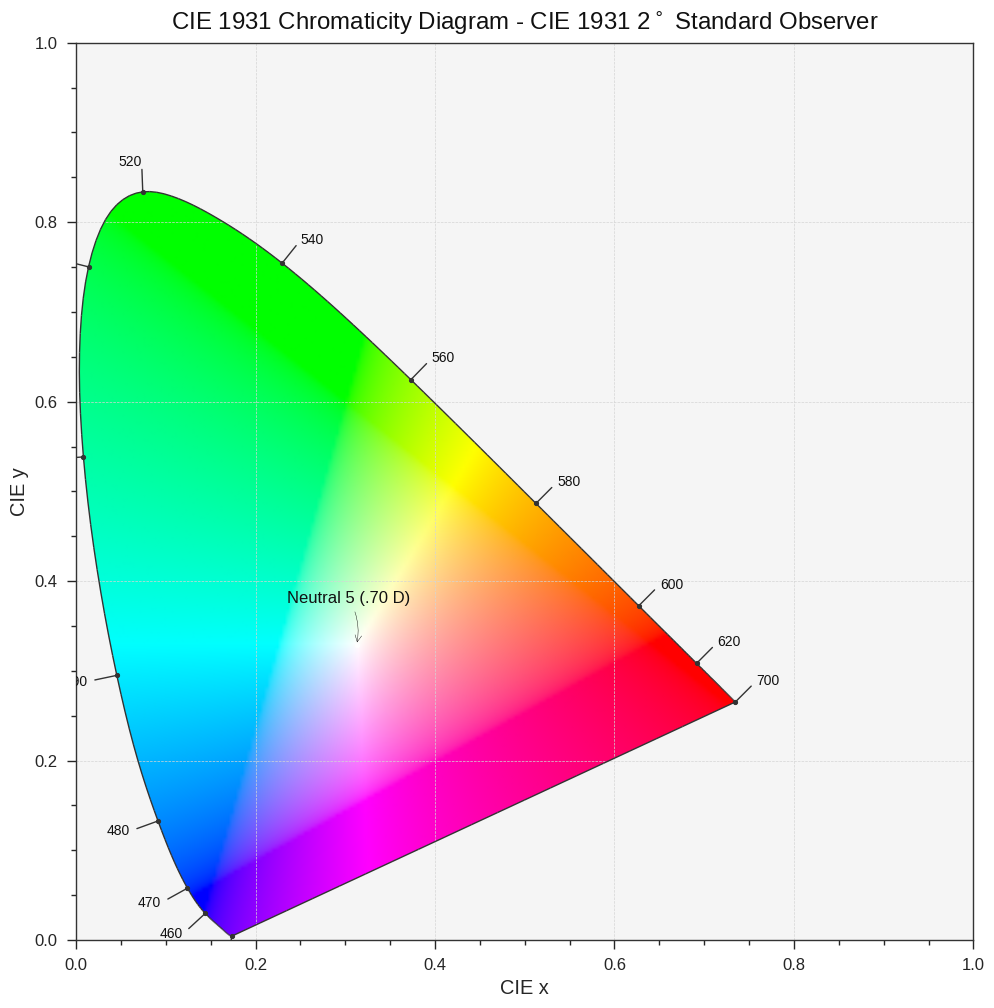
\includegraphics[width=\linewidth]{img/cie.png}
  \caption{CIE 1931 Chromaticity Diagram from \cite{mansencal_thomas_2018_2647615}}
  \Description{Spectral locus}
\end{figure}

Embedding an understanding of both linear space and gamma space into our workflow, could significantly change the very aesthetic of the images when viewed with color gamuts of digital displays, as such, should have an impact on the experience on the produced digital hologram.  One way to test these differences in our proposed pipeline is to test the making our image stack by incorporating the above stated factors in our production.

\\
\subsection{Digital Holograms}

% --------------------------------------------------------------
% Results
% --------------------------------------------------------------
\newpage
\section{Results}
Similarly to method section, this section will be divided into 4 main sections: segmentation, generating 3D models or geometry, image stage generation, and finally digital holograms. 





\subsection{Segmentation}
In our data set there were 181 slices each containing and image with the dimensions 256x256.  For each slice the segmentation described in the segmentation section of the report was performed to identify each of the known tissues within our dataset.  Figure \ref{fig:resultsHistogram} shows an example the histogram distribution along with their corresponding MRI. Note the distinct peaks of the histogram which corresponds the the distinct known tissues of the brain.\\ 

\begin{figure}[H]
  \centering
  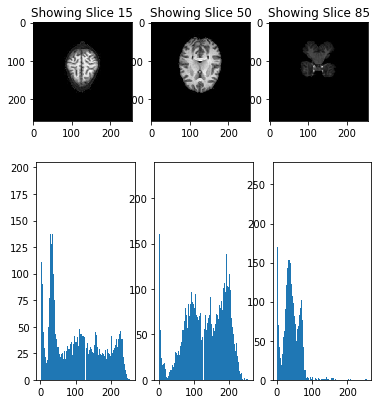
\includegraphics[width=\linewidth]{img/resultsHistogram.png}
  \caption{Brain slices of MRI with their corresponding histogram distribution.}
  \label{fig:resultsHistogram}
\end{figure}

Results of the manual seed region growing techniques and morphological filters can be seen in figure \ref{fig:resultsSegmentation}.

\begin{figure}[H]
  \centering
  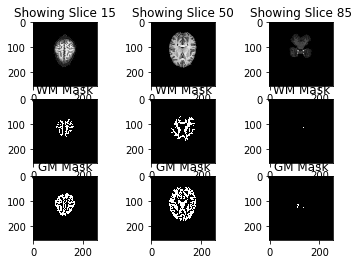
\includegraphics[width=\linewidth]{img/resultsSegmentation.png}
  \caption{\textbf{Top Row:} Original MRI. \textbf{Middle Row:}White matter mask. \textbf{Bottom Row:}Gray matter mask.}
  \label{fig:resultsSegmentation}
\end{figure}

We applied this technique not only for the regular brain but also for a brain which contains a tumor.  The following set of figures shows examples slices as well as their resultant class labels and individual mask layers.

\begin{figure}[H]
  \centering
  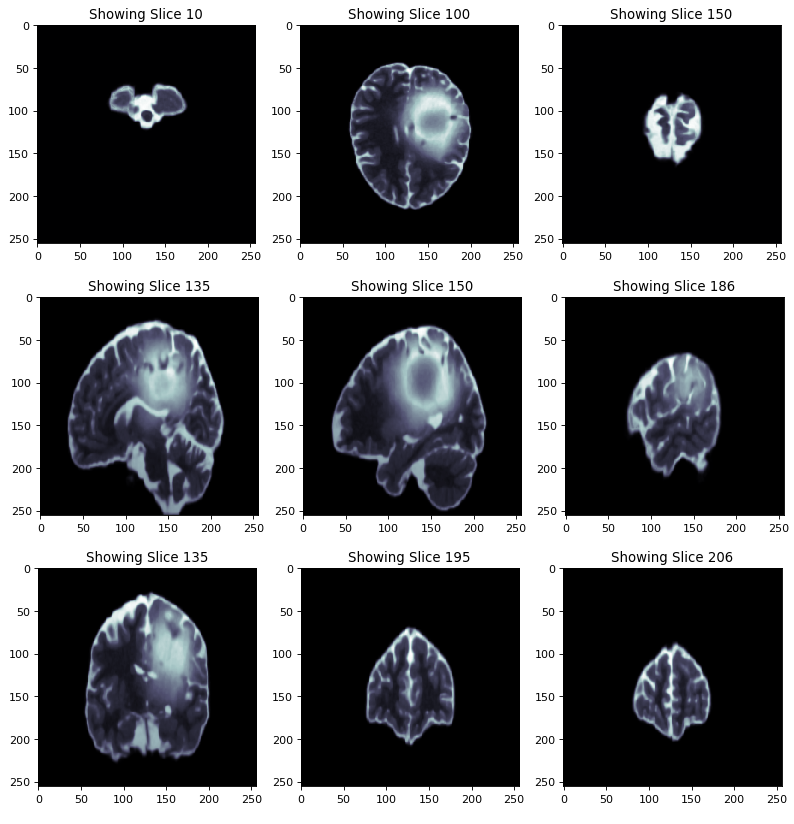
\includegraphics[width=\linewidth]{img/originalMRI.png}
  \caption{Original MRI slices in different views.  From top to bottom they are sliced in the axial, sagittal and coronal planes.}
  \label{fig:originalMRI}
\end{figure}

Note: the following images might look distorted and they are, and the reason is that because we have limited number of slices interpolation must be done to resize the image to its original width and height. Note the deformation of the coronal and sagittal views because of the limited depth data. Regardless I think we can use these views to narrow down the slices of interest.

\begin{figure}[H]
  \centering
  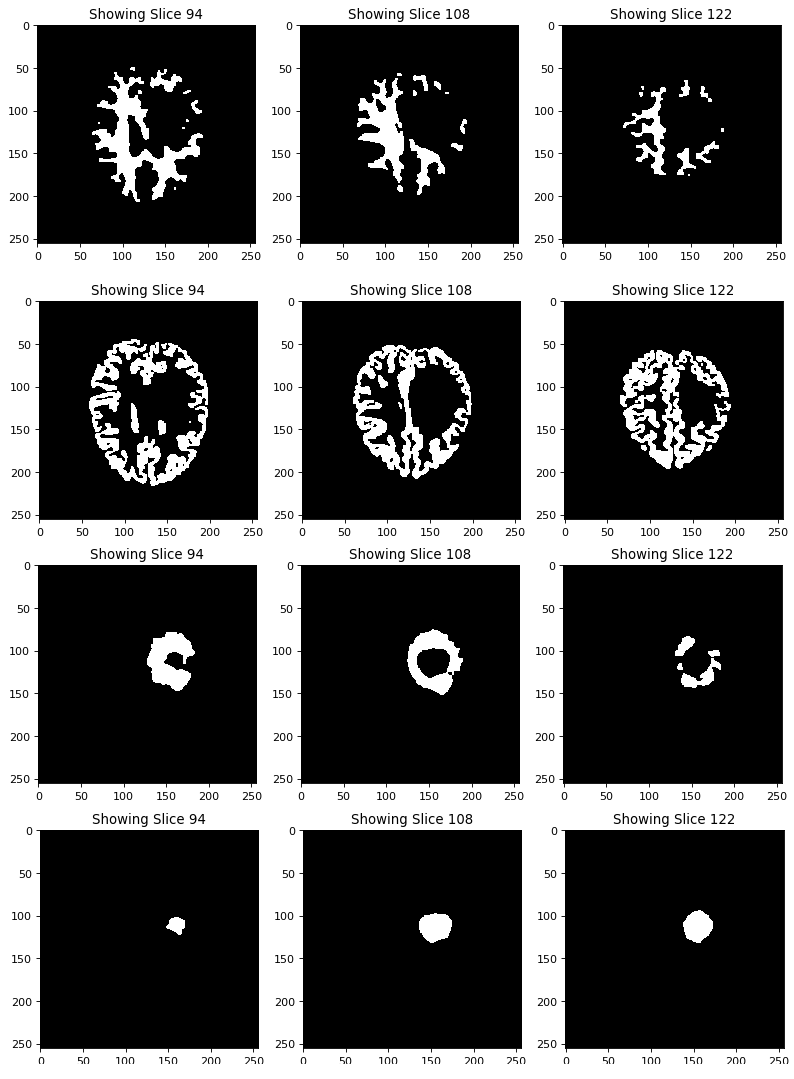
\includegraphics[width=\linewidth]{img/resultantMasks.png}
  \caption{Generated masks for each of the known tissue classes in our dataset.  From top to bottom they are: gray matter, white matter, abnormal tissue, and tumor.}
  \label{fig:resultantMasks}
\end{figure}

Even though we applied morphological filters we can still see some noise within the images, specifically the speckle effects in the gray matter and some holes in the white matter masks.  We can manually remove this again we can't because we can't modify data.

\begin{figure}[H]
  \centering
  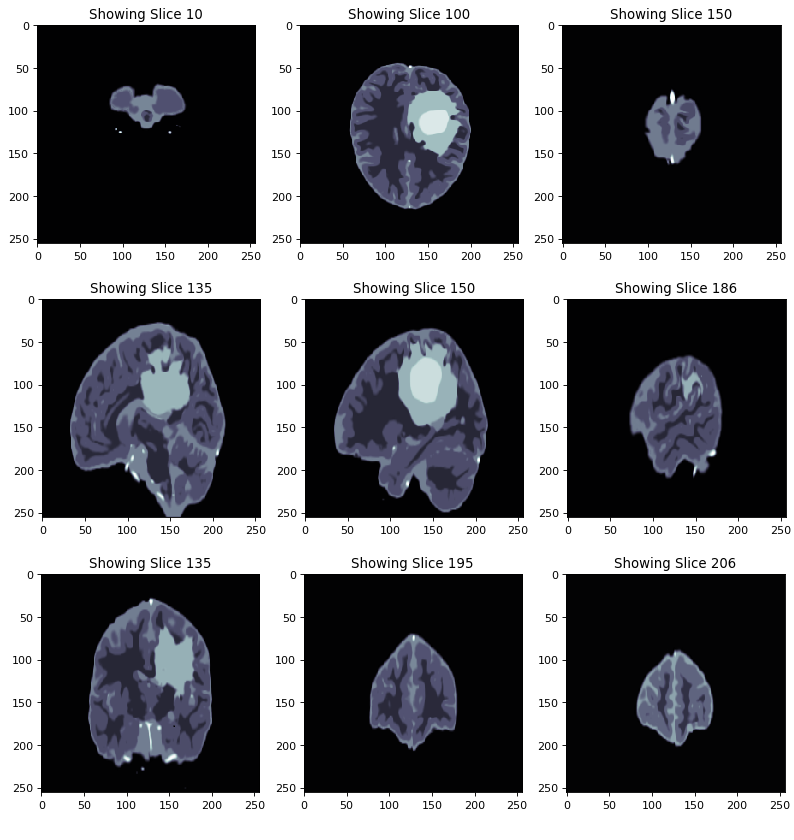
\includegraphics[width=\linewidth]{img/labeledMasks.png}
  \caption{Various slices and views of each of the coloured masks as found in the histogram.}
  \label{fig:labeledMasks}
\end{figure}

Each unique colour corresponds to a unique known tissue type.  By looking at various views you can get a picture as to where to tumor maybe located.  To create contrast between each distinct region we proposed the following colouring scheme.

\begin{figure}[H]
  \centering
  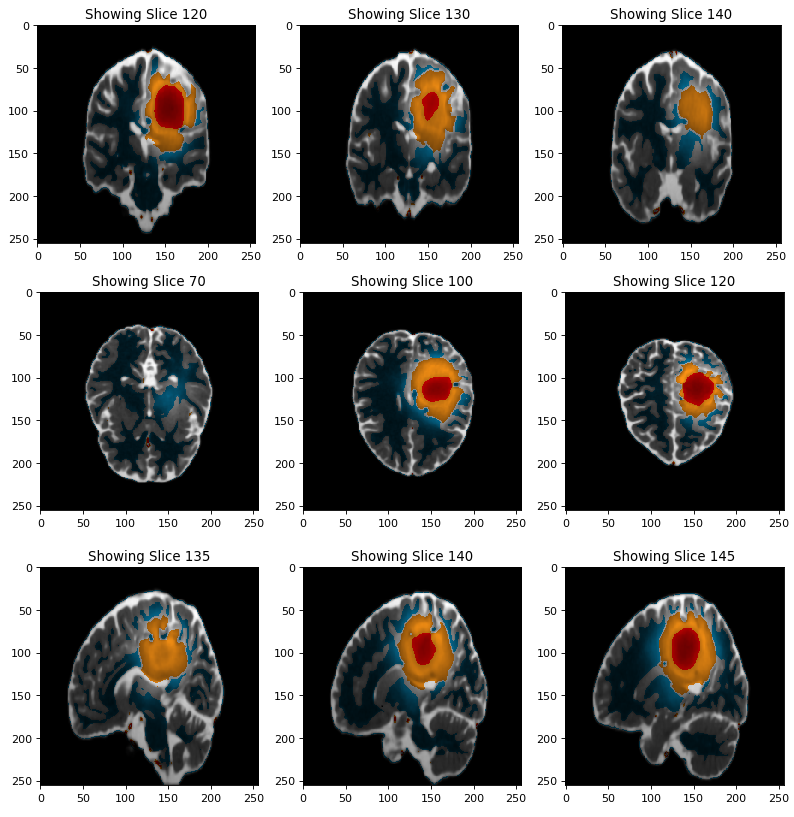
\includegraphics[width=\linewidth]{img/colourCodedRegions.png}
  \caption{}
  \label{fig:colourCodedRegions}
\end{figure}

\begin{table}[h]
\centering
\begin{tabular}{|r|l|l|l|}
\hline
Tissue & R & \multicolumn{1}{c|}{G} & B \\ \hline
White & 7 & \multicolumn{1}{c|}{150} & 204 \\ \hline
Gray & 204 & 204 & 204 \\ \hline
Abnormal Tissue & 203 & 119 & 17 \\ \hline
Tumor & 203 & 2 & 2 \\ \hline
\end{tabular}
\caption{undefined}
\label{undefined}
\end{table}

Notice that for each of the tissue types they can be clearly distinguish from each other. 
\subsection{Generating Geometry}

\subsubsection{Marching Cube Algorithm}

\subsubsection{Marcus Method}

\subsubsection{Jawa Method}
\subsection{Frame Stack Generation}
\begin{figure}[H]
  \centering
  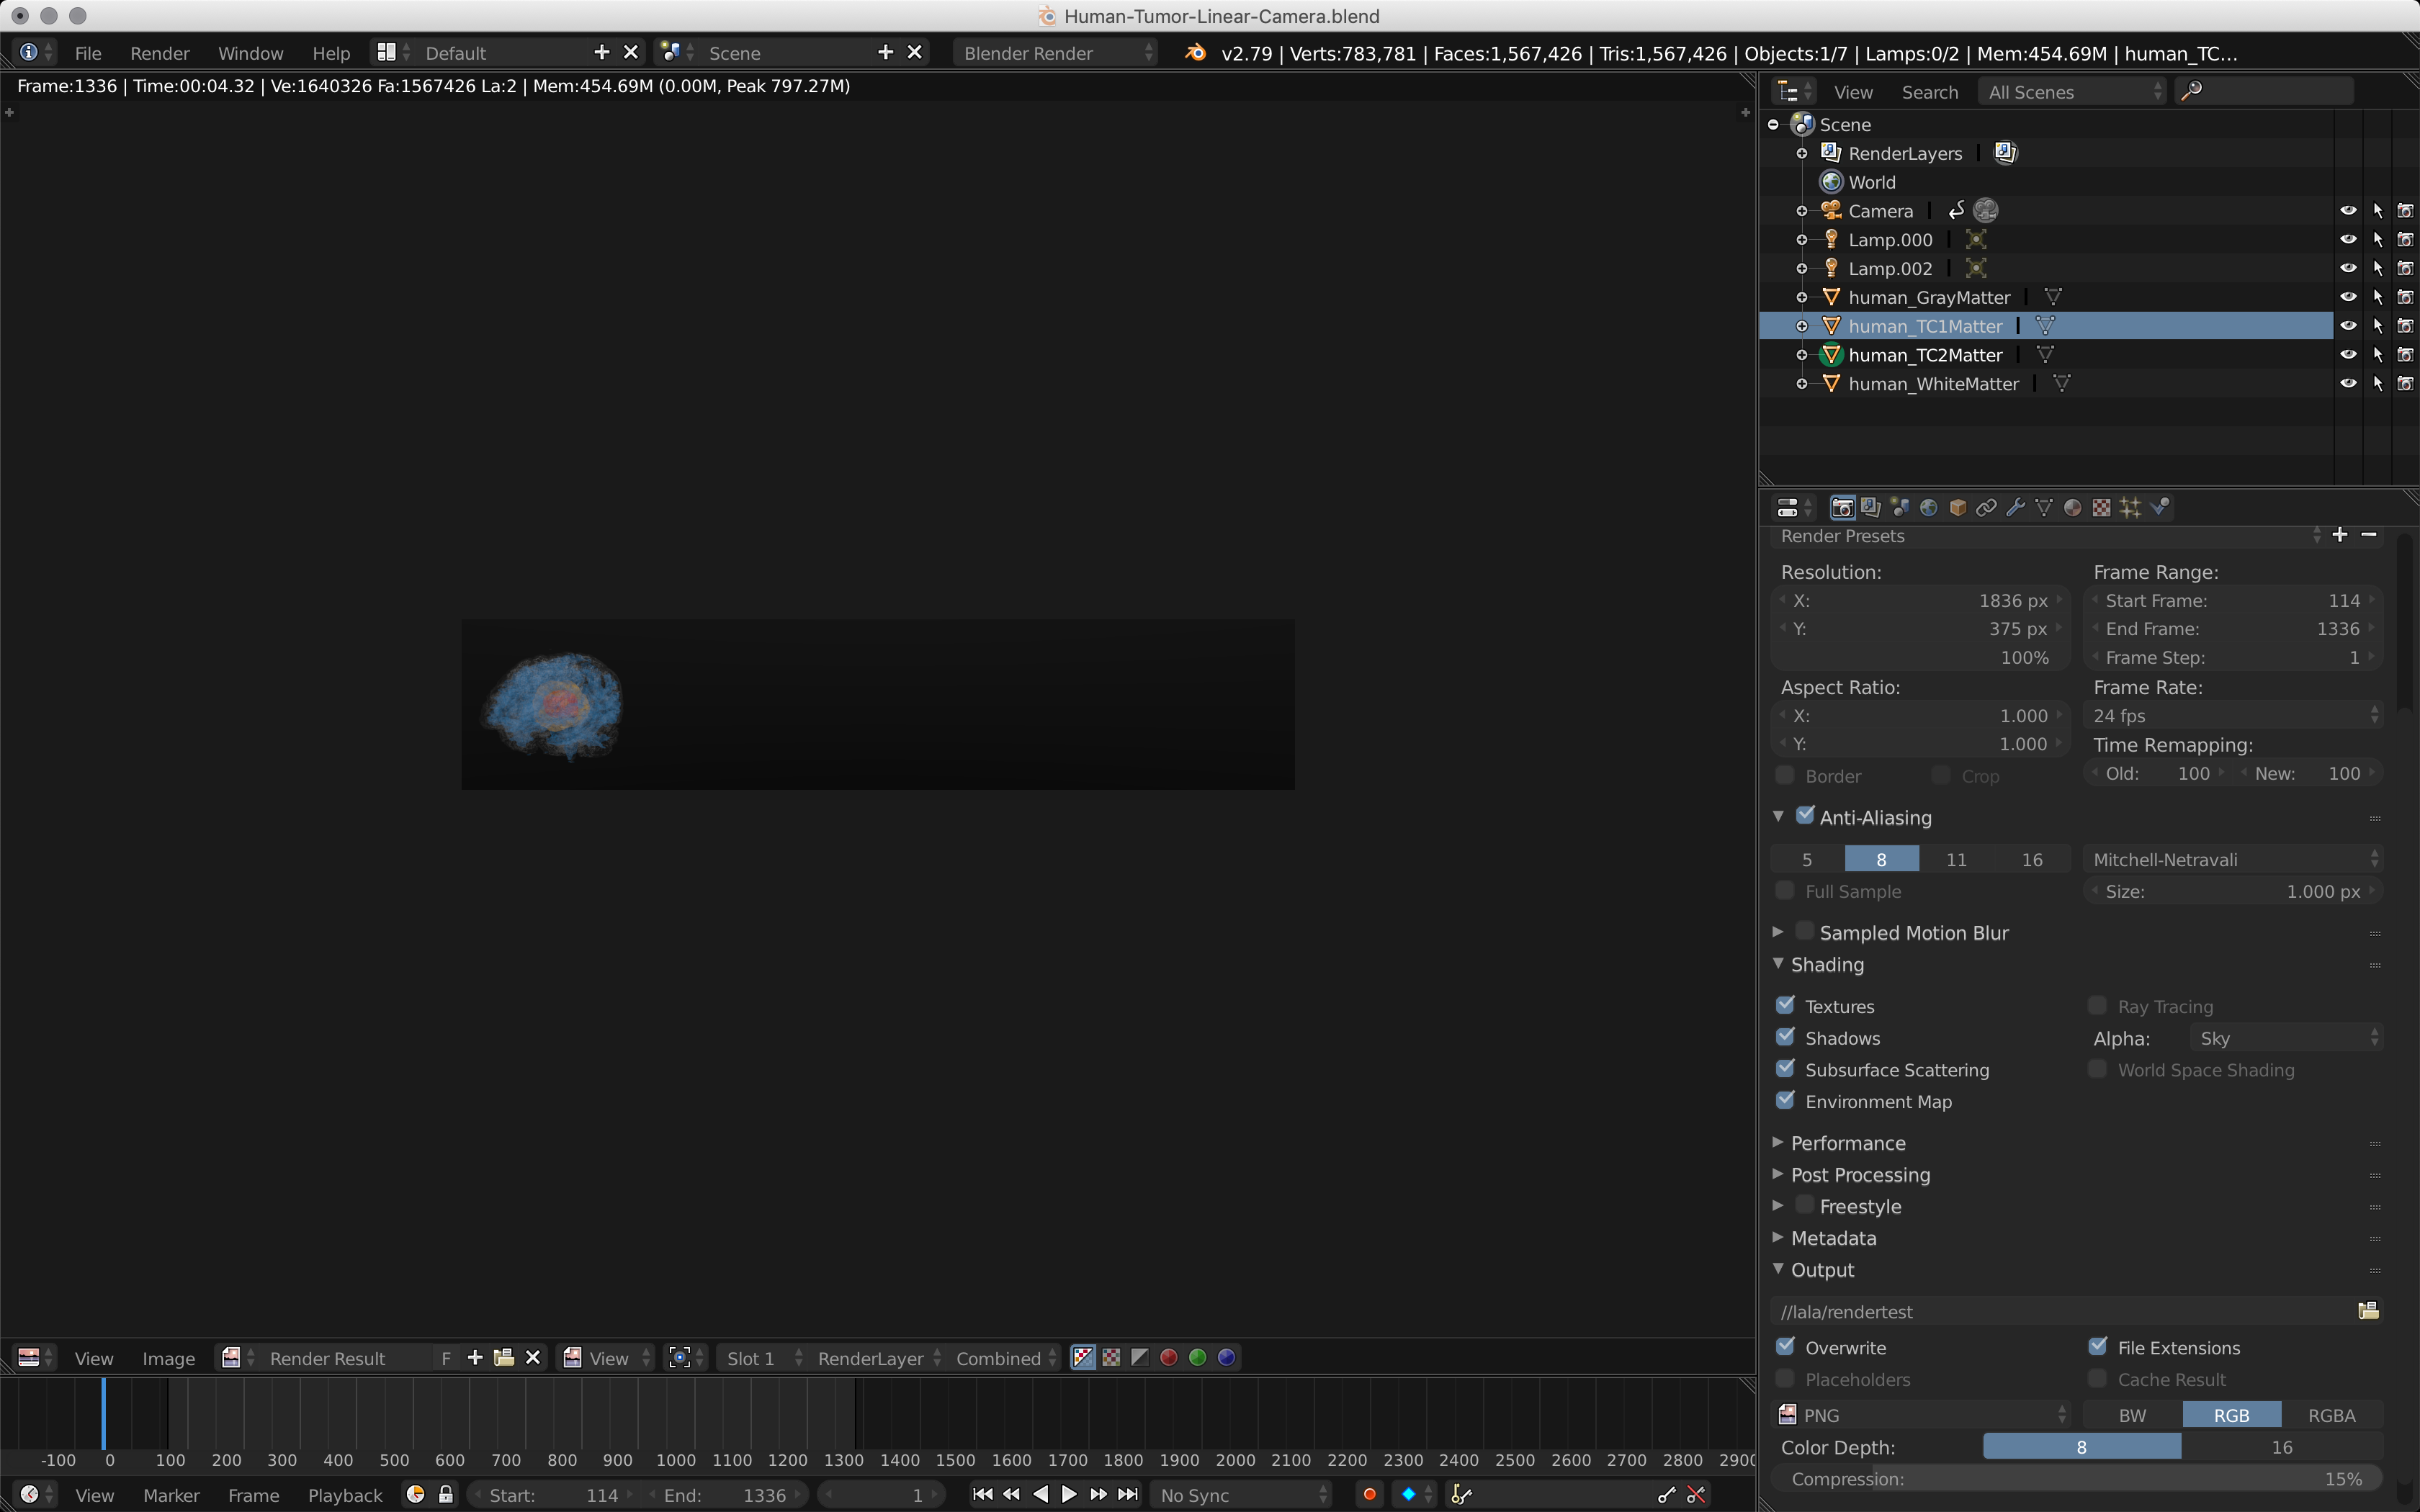
\includegraphics[width=\linewidth]{img/linCam1.png}
  \caption{Blender view of linear camera setup. Image by Marcus A. Gordon.}
  \Description{Blender view of linear camera setup}
\end{figure}

In order to develop our digital hologram, we create a virtual camera setup that mimics the recording behaviour of our holographic printer.  We call this virtual camera setup the `linear camera' as it refers to the linear movement of photographing the three dimensional space from right to left.  This virtually photographed three dimensional space becomes the field of view of the observer of the hologram and holds the dimensionality and depth of the objects in its scene within 1336 angles of view.

The viewing window set for this is 1836px by 375px as shown in Figure 10.


\subsection{Digital Holograms}

% --------------------------------------------------------------
% Discussion
% --------------------------------------------------------------
\newpage
\section{Discussion}

% --------------------------------------------------------------
% Conclusion and Future Work
% --------------------------------------------------------------
\newpage
\section{Conclusion and Future Work}

% --------------------------------------------------------------
% Appendix
% --------------------------------------------------------------
\newpage
\section{Appendix}
\appendix
\section{Python Functions for The Implementation of Semi-Automatic Segmentation and Model Generation}
\label{sec:appendixPythonFunction}

\lstinputlisting[language=python,caption=All python functions pertaining to semi-automatic segmentation and model generation.]{sections/code/Human_TumorSegmentationFunction.py}
\section{Python Main Code for The Implementation of Semi-Automatic Segmentation and Model Generation}
\label{sec:appendixPythonMain}

\lstinputlisting[language=python,caption=Python main program pertaining to semi-automatic segmentation and model generation.]{sections/code/Human_TumorSegmentationMain.py}


% --------------------------------------------------------------
% Bibliography
% --------------------------------------------------------------
\newpage
\section{Bibliography}
\bibliography{sample-base.bib}
\bibliographystyle{acm}
\newpage

\end{document}
